\documentclass[a4paper,11pt]{article}
\oddsidemargin 0.0cm  
\evensidemargin 0.0cm  
\textwidth 17cm 
\topmargin -1cm 
\textheight 23.5cm
\usepackage{graphicx}
\usepackage{float} 
\usepackage{multimedia}
\usepackage{amsmath,amssymb}
\usepackage{listings}
\usepackage{graphicx} % Allows including images
\usepackage{booktabs} % Allows the use of \toprule, \midrule and \bottomrule in tables

\usepackage{scrextend}
\usepackage{amsfonts}
\usepackage{amsmath,bm}
\usepackage{algorithm}
\usepackage{algorithmic}
\usepackage{graphicx}
\usepackage[round]{natbib}
\lstset{
  numbers=left,   
  firstnumber=1,
  numberfirstline=true,
  language=C, 
  frame=L
  } 

\title{Internship: Inverse Procedural Generation of Geological Stories}
\author{Maxime Garcia}
\date{\today}

\begin{document}
\maketitle
\section{Context}

%Hand sketching 2D sections of the soil allows geologists to illustrate and validate their hypothesis about recorvering its history. Their assumptions are based on geological knowledge and rules. Moreover by looking at the different layers and faults, the geologist is able to expand or compress the soil to represent what it was like before sedimentation, erosion and tectonic movements.
%The resulting drawing is called a reconstitution. \\\\
%However this approach is rather limited because it only takes into account the soil history at discrete steps and doesn't necessarily keep the drawing cohesion between two steps.
%Recently a new numerical sketching method was proposed [1]. It organizes geological sketches into story trees allowing to compare different interpretations of the soil history . This method allows the geologist to draw over the previous frame in order to help him keep the drawing consitency. It allows also to draw several hypothesis that lead to the same soil configuration and play the animation of those at the same time for comparing them.
%However even if such a method can help geologist beeing more consistant and clearer about their hypothesis, we can't visualize the full geological history that a continuous animation can provide.\\\\
%Our approach is centered on this continuous animation aspect.
%Concretely starting from the 2D current section of the soil we will create automatically a story tree containing all plausible animation scenarios that generated the current soil situation. After generating the tree it will be possible to play the animation starting from the leaves and visualize the forward creation of our 2D current section.


Hand-drawn sketches are useful in geology for illustrating and validating hypotheses. Moreover by looking at the different layers and faults, the geologist is able to expand or compress the soil to represent what it was like before sedimentation, erosion and tectonic movements. The resulting drawing is called a restoration.\\\\
However those drawings are rather limited. On top of representing only one 2D slice of the terrain being investigated, they can only represent hypotheses on the underground composition at discrete time steps, rather than a complete history. 
In addition insuring consistency between these sketches over time heavily depends on the skills of the geologist, and on his knowledge on the way geologic slices of soil fold, on the way cracks propagates and produce sliding, and on the way sediments are deposited.\\\\ 
Exploring different hypotheses is very difficult, if not impossible, with the current pipeline.
Recently, it was proposed to organize geological sketches into « story trees » to present and
compare different interpretations of the formation of a given terrain [1] but the task remains
labor-intensive, requiring the geologist to draw every sketch in the story tree. \\\\
In this internship, we would like to follow up on this line of research by proposing methods for inferring a
geological story tree directly from very few geological sketches, and presenting the resulting tree of
possible geological stories as an animation.

\section{Objectives}

Our approach will focus on providing a continuous animation of the geological story computed automatically from a geologist sketch drawn with \textbf{vpaint} software [2]. \\\\
Our main objective is to produce an inverse modeling animation rather than a forward modeling one like state of the art methods for geological restoration validation can provide.\\
In addition we have to decompose the geological story into discrete events (such as faults) and continuous ones (such as erosion and sedimentation). Thus we propose a tree structure to encode this story.\\\\
Finally the animation will be created on top of \textbf{vpaint} software which takes into account the topological changes due to discrete events as well as the effect of continuous events in time.

\section{State of the art}

Like mentioned above, several continuous animation tools for soil evolution in time are already available.
They work on the assumption that sedimantary layers were in a horizontal configuration at the starting position which is a well used hypothesis in geology. 
With this assumption sofware such as SLAMTec or OptumG2 offer the possibility to mechanically simulate the compression of a sedimental section.\\\\
The goal of this kind of forward simulation is to validate a restoration that had been generated from a present dating 2D section and see if the result coincidates with it. This kind of simulation is configurable by several factors such as the erosion and the friction coefficients.\\\\
Soil restoration can be obtained thanks to geometrical tools. Those tools deal with each block (soil section between two faults) one by one and flatten each layer while conserving their respective area. After the flattening operation the user can manually stick the new block to its neighbours with the corresponding layers facing each other. 
Here is an example of restoration taken from Chartreuse slice:

\begin{figure}[H]
\centering
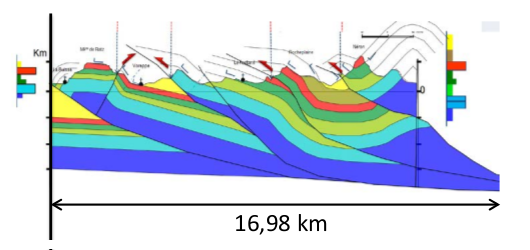
\includegraphics[scale=0.9]{Wraped_Section.png}
\caption{Current slice of Chartreuse soil}
\end{figure}

\begin{figure}[H]
\centering
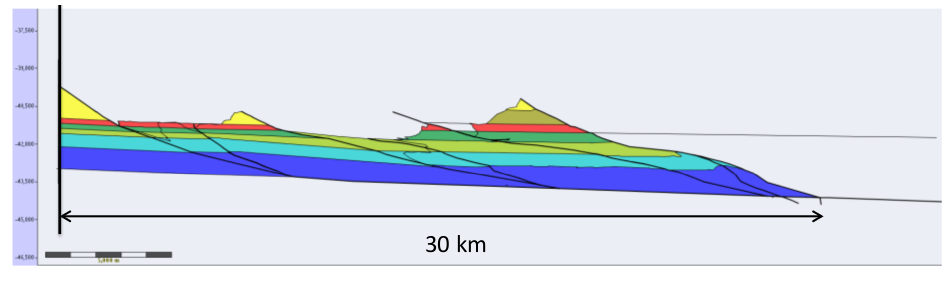
\includegraphics[scale=0.7]{UnWraped_Section.png}
\caption{Restoration of Chartreuse soil}
\end{figure}

As this restoration is done manually by a geologist it corresponds to a plausible past state of the soil where we can run forward simulation on it to actually compare with the current section and validate it. \\\\

\section{Our approach}

Unlike forward animation techniques which use a restoration and run a mechanical simulation over it, we will run an inverse modeling animation on the current 2D section and compare it visually to the provided restoration. 
In order to explore a reasonable number of history scenarios we will encode them into an interactive story tree.\\\\
We first provide one possible scenario to the user making the story tree taking the form of a line. Starting from that point the user can decide to create another branch from any node and explore a new scenario. 
%By proceeding this way we can restrict the number of scenario we will propose to the user as he is controlling that number himself. 
Each node of the tree will corresponds to a discrete topological event sush as faults, meaning that between two consecutive node levels we will simulate the consequence of this event. Thus the tree banches will correspond to the continuous animation of the soil change caused by the end node event of the branch. \\\\
However discrete geological events are not the only phenomena we have to consider in order to represent all the plausible scenarios. Indeed continuous events such as erosion and sedimentation have to be taken into account. Those events will be integrated into the tree as branches.\\
More phenomena may be added during the internship but we have to be careful to not produce too many scenarios that are not relevent, therefore the number of considered phenomena should be moderated.
However the number of unrelevent scenarios can be reduced by taking into account more geological laws that will restrict node and branch creations.\\
Thus at each node and branch creation, the user can only choose events among a restricted range. This property is important because it is time saving for geologists who want to see just the most plausible scenarios.\\\\
Before genarating the tree we will extract all the information we can from the 2D section, that is to say the number of layers, their age, the already determined eroded zones and so on.\\\\
As geological structures can have a rather complex topology, the 2D section will be presented as a vector graphics complex representation [3] drawn using \textbf{vpaint} software like in Figure 3. This data structure has been shown to model all possible incidence relations between vertices, edges and faces in 2D sketches. More structures derivating from vector graphics complex will be implemented in order to take into account the geological aspect of the sketch.\\\\
The inverse modeling animation will be done on top of the vector animation complex structure [4] which is used to describe all possible changes in the topology of a vector graphic complex over time.
This method will require prior information about several geological parameters that will affect the animation such as materials' density, friction coefficients and others like erosion and sedimentation speeds.


\begin{figure}[H]
\centering
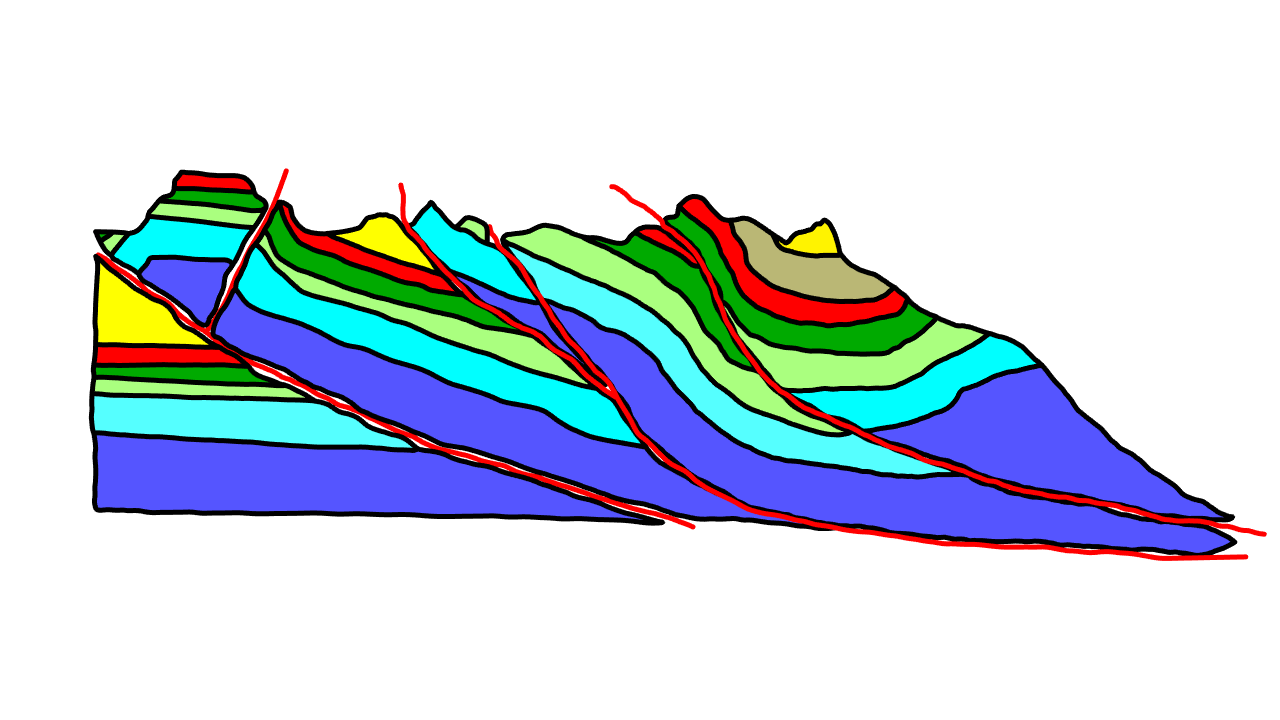
\includegraphics[scale=0.5]{chartreuse_paint.png}
\caption{Vpaint drawing of chartreuse slice}
\end{figure}

\section{Validation}

The validation will be done in a subjective way by experts. The model concistancy and reliability will be evaluated visually.
In addition the experts can provide us unit tests using analogic simulation with sand boxes.
%The validation will be done by analogic simulations of a real soil with sand boxes. Sedimental layers are disposed in an horizontal manner in order to represent the starting point which corresponds to the reconstruction. Then compression or extension is applied to one or both sides of the box in order to simulate the topological changes in a short time. In addition erosion can be applied by  removing matter from the box. This technique can be used to make unit test in our simulations, for instance when testing only the fault sliding or the erosion effect.

\section{References}

[1] Lidal, Endre Mølster; Natali, Mattia; Patel, Daniel; Hauser, Helwig; Viola, Ivan.
Geological storytelling. Computers \& graphics. 37: 445-459.\\

\noindent[2] http://www.vpaint.org/ \\

\noindent[3] Boris Dalstein, Remi Ronfard, Michiel Van De Panne. Vector Graphics Complexes. ACM transactions on
Graphics, Proceedings of ACM SIGGRAPH 2014.\\

\noindent[4] Boris Dalstein, Remi Ronfard, Michiel van de Panne. Vector Graphics Animation with Time-Varying Topology.
ACM Transactions on Graphics, 34, 4, Proceedings of ACM SIGGRAPH 2015.


\end{document} 